\begin{frame}{Detection: 1D-DBSCAN over Sorted Keys}
    \ourbadge
    \begin{columns}[T,onlytextwidth]
        \column{0.60\textwidth}
        \textbf{Goal:} find segments dense enough to fit exact mode
        at fingerprint width $K = \lceil\log_2(n\mathcal{L}/\varepsilon)\rceil$
        \medskip

        \begin{itemize}
                    \setlength{\itemsep}{0.3em}
                \item One-pass scan over sorted keys, $O(n)$.
                \item DBSCAN (density-based clustering) predicate, radius derived from $K$.
                \item Span $\le 2^K \Rightarrow$ exact ERE (FPR $= 0$);
            else $\Rightarrow$ fallback.
                \item Threshold derived from problem geometry.
        \end{itemize}

        \column{0.40\textwidth}
        \vspace*{3em}
        \centering
        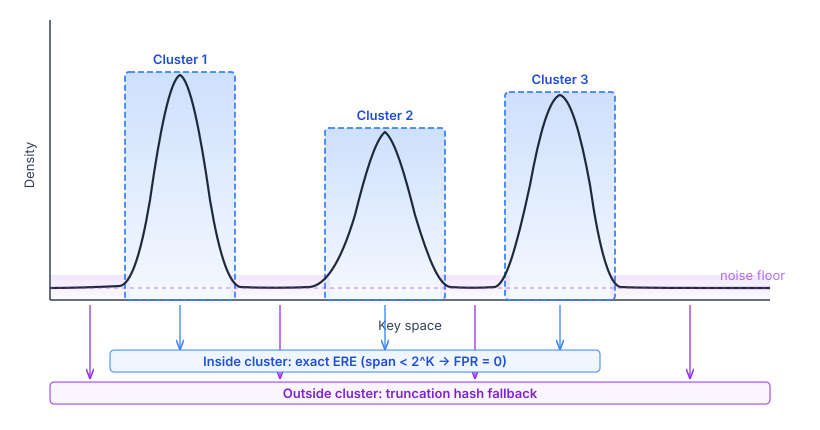
\includegraphics[width=\linewidth, keepaspectratio]{../../figures/segmentation}
        \vspace*{\fill}
    \end{columns}
\end{frame}
